\documentclass{wileySix}

\usepackage{graphicx}
\usepackage{listings}

\usepackage{color}
 
\definecolor{codegreen}{rgb}{0,0.6,0}
\definecolor{codegray}{rgb}{0.5,0.5,0.5}
\definecolor{codepurple}{rgb}{0.58,0,0.82}
\definecolor{backcolour}{rgb}{0.95,0.95,0.92}
 
\lstdefinestyle{mystyle}{
    backgroundcolor=\color{backcolour},   
    commentstyle=\color{codegreen},
    keywordstyle=\color{magenta},
    numberstyle=\tiny\color{codegray},
    stringstyle=\color{codepurple},
    basicstyle=\footnotesize,
    breakatwhitespace=false,         
    breaklines=true,                 
    captionpos=b,                    
    keepspaces=true,                 
    numbers=left,                    
    numbersep=5pt,                  
    showspaces=false,                
    showstringspaces=false,
    showtabs=false,                  
    tabsize=2,
    language=TeX,
	caption=Coy kasih caption dong,
	label={lstlisting_nya_ada_yang_belum_dikasih_label}
}
 
\lstset{style=mystyle}

\usepackage{w-bookps}

\setcounter{secnumdepth}{3}

\setcounter{tocdepth}{2}


\docropmarks


\newcommand{\VT}[1]{\ensuremath{{V_{T#1}}}}


\newbox\sectsavebox
\setbox\sectsavebox=\hbox{\boldmath\VT{xyz}}



\begin{document}


\booktitle{Cerdas Menguasai Latex}
\subtitle{Dalam 24 Jam}

\authors{Rolly M. Awangga\\
\affil{Informatics Research Center}}

\offprintinfo{Cerdas Menguasai Latex, First Edition}{Rolly M. Awangga}


\halftitlepage

\titlepage


\begin{copyrightpage}{2019}
%Survey Methodology / Robert M. Groves . . . [et al.].
%\       p. cm.---(Wiley series in survey methodology)
%\    ``Wiley-Interscience."
%\    Includes bibliographical references and index.
%\    ISBN 0-471-48348-6 (pbk.)
%\    1. Surveys---Methodology.  2. Social 
%\  sciences---Research---Statistical methods.  I. Groves, Robert M.  II. %
%Series.\\
%
%HA31.2.S873 2007
%001.4'33---dc22                                             2004044064
\end{copyrightpage}

\dedication{`Jika Kamu tidak dapat menahan lelahnya belajar, 
Maka kamu harus sanggup menahan perihnya Kebodohan.'
~Imam Syafi'i~}

\begin{contributors}
\name{Rolly Maulana Awangga,} Informatics Research Center., Politeknik Pos Indonesia, Bandung,
Indonesia



\end{contributors}

\contentsinbrief
\tableofcontents
\listoffigures
\listoftables
\lstlistoflistings


\begin{foreword}
Sepatah kata dari Kaprodi, Kabag Kemahasiswaan dan Mahasiswa
\end{foreword}

\begin{preface}
Buku ini diciptakan bagi yang awam dengan git sekalipun.

\prefaceauthor{R. M. Awangga}
\where{Bandung, Jawa Barat\\
Februari, 2019}
\end{preface}


\begin{acknowledgments}
Terima kasih atas semua masukan dari para mahasiswa agar bisa membuat buku ini 
lebih baik dan lebih mudah dimengerti.

Terima kasih ini juga ditujukan khusus untuk team IRC yang 
telah fokus untuk belajar dan memahami bagaimana buku ini mendampingi proses 
Intership.
\authorinitials{R. M. A.}
\end{acknowledgments}

\begin{acronyms}
\acro{ACGIH}{American Conference of Governmental Industrial Hygienists}
\acro{AEC}{Atomic Energy Commission}
\acro{OSHA}{Occupational Health and Safety Commission}
\acro{SAMA}{Scientific Apparatus Makers Association}
\end{acronyms}

\begin{glossary}
\term{git}Merupakan manajemen sumber kode yang dibuat oleh linus torvald.

\term{bash}Merupakan bahasa sistem operasi berbasiskan *NIX.

\term{linux}Sistem operasi berbasis sumber kode terbuka yang dibuat oleh Linus Torvald
\end{glossary}

\begin{symbols}
\term{A}Amplitude

\term{\hbox{\&}}Propositional logic symbol 

\term{a}Filter Coefficient

\bigskip

\term{\mathcal{B}}Number of Beats
\end{symbols}

\begin{introduction}

%% optional, but if you want to list author:

\introauthor{Rolly Maulana Awangga, S.T., M.T.}
{Informatics Research Center\\
Bandung, Jawa Barat, Indonesia}

Pada era disruptif  \index{disruptif}\index{disruptif!modern} 
saat ini. git merupakan sebuah kebutuhan dalam sebuah organisasi pengembangan perangkat lunak.
Buku ini diharapkan bisa menjadi penghantar para programmer, analis, IT Operation dan Project Manajer.
Dalam melakukan implementasi git pada diri dan organisasinya.

Rumusnya cuman sebagai contoh aja biar keren\cite{awangga2018sampeu}.

\begin{equation}
ABC {\cal DEF} \alpha\beta\Gamma\Delta\sum^{abc}_{def}
\end{equation}

\end{introduction}

%%%%%%%%%%%%%%%%%%Isi Buku_

\chapter{Editor dan Compiler}
\section{Mengenal .tex}
Pertama pahami dulu bagaimana badan isi file .tex yang akan kita kerjakan. Download atau lihat salah satu file latex yang akan kita kerjakan. Untuk mengisi latex kita harus mengisinya di dalam komponen \textit{document} yang merupakan tag dengan pembuka begin dan diakhiri dengan end.
Kemudian kenali bagian buku terdiri dari part, chapter dan section. Part itu bisa kita andaikan bab, chapter sub bab, dan section adalah bagian.

Kita bisa memisahkan isi dari latex dengan perintah input kemudian di dalam kurung kurawal letak file .tex yang akan kita masukkan kedalam file utama latex tersebut.

\section{Compiler}
Pastikan kita sudah install aplikasi editor latex. Disini saya praktekkan menggunakan texmaker. Kita bisa melakukan kompilasi dengan perintah yang ada di listing \ref{lst:compile}.

\begin{lstlisting}[caption=Perintah kompilasi latex keluaran pdf,label={lst:compile},language=sh]
pdflatex -shell-escape -interaction=nonstopmode -file-line-error git.tex | grep ".*:[0-9]*:.*|LaTeX Warning:"

pdflatex -shell-escape -interaction=nonstopmode -file-line-error git.tex | grep ".*:[0-9]*:.*"

pdflatex -shell-escape -interaction=nonstopmode -file-line-error git.tex | grep -i ".*:[0-9]*:.*\|warning"
\end{lstlisting}

\chapter{Pengaturan Paragraf}
\section{Pembagian bab}
Secara default pembagian bab pada latex menggunakan perintah \textit{section}, \textit{subsection}, \textit{subsubsection} dan \textit{subsubsubsection}. Untuk mengatur kedalaman suatu dokumen pada bab bab tertentu, kita dapat menggunakan perintah berikut ini pada bagian Preamble :
setcounter.secnumdepth
setcounter.tocdepth


Opsi yang digunakan pada syntax secnumdepth pada perintah verbcounter= seperti perintah diatas, berarti Anda telah merubah kedalaman bab yang Anda perbaharui sampai dengan level 5 yaitu section -- subsection -- subsubsection -- paragraph -- subparagraph. Sedangkan pada perintah dari opsi tocdepth berfungsi untuk membuat table of contents atau menampilkan kedalaman bab sampai dengan level 5, namun jika tidak di setel maka pada bagian level 3 kebawah tidak akan dapat ditampilkan pada bagian toc \ref{labelgambar}.
\begin{figure}[ht]
\centerline{\includegraphics[width=1\textwidth]{figures/capture.JPG}}
\caption{Pembagian Bab.}
\label{labelgambar}
\end{figure}



\section{Format Cetak}
Pada format LateX teks mempunyai bentuk plaintext, yang artinya teks tersebut belum diformat. Pada proses formatting teks dapat dilakukan dengan bahasa tersendiri yaitu bahasa markup. Hal paling mendasar antara lain cetak tebal, miring dan gari bawah. Cetak tebal menggunakan perintah \textit{textbf},cetak miring menggunakan perintah \textit{textit} dan garis bawah menggunakan perintah \textit{underline}.

\section{Tanda petik}
Tanda petik di Latex menggunakan petik miring dan petik satu. Petik miring biasanya berada pada sebelah angka satu di keyboard dan diakhiri petik satu. Ingat fungsi tanda petik hanya untuk melakukan quote atau pengutipan langsung. Untuk istilah bahasa inggris gunakan miring atau italic.

\begin{lstlisting}[caption=Contoh kalimat dalam tanda petik pada Latex,label={lst:tandapetik}]
`kalimat dalam tanda petik'
\end{lstlisting}

\section{Penomoran}
Perintah penomoran pada latex biasanya menggunakan format \textit{Numbering} atau format \textit{Bullets}. Perintah yang digunakan pada format Numbering adalah \textit{enumerate} sedangkan untuk Bullets yang menyerupai poin menggunakan \textit{itemize}.

\textit{Numbering} merupakan perintah yang digunakan untuk membuat daftar berurut dengan penomoran menggunakan angka (numbered list), yang biasanya diberikan pada awal baris baru \ref{lst:PenomoranNumbering}. 
\lstinputlisting[caption=Memberikan Perintah Numbering,label={lst:PenomoranNumbering}]{src/1/lstlistingNumbering.tex}
Sedangkan \textit{Bullets} atau poin adalah perintah yang digunakan untuk membuat daftar berurut dengan penomoran berupa symbol atau poin (bulleted list) \ref{lst:penomoran}.
\lstinputlisting[caption=Menambahkan kode perintah bullets,label={lst:penomoran}]{src/1/poin.tex}


\section{Karakter Khusus}
Untuk memberikan karakter khusus pada LaTex kita dapat menggunakan tanda \textit{backslash} didepan karakter yang ingin kita tandai. Terdapat beberapa karakter yang tidak bisa langsung digunakan seperti tanda \textit{ampersand}. Selain itu format pemberian kutipan pada LaTex berbeda dengan pemberian kutipan pada editor lainnya seperti pada gambar \ref{KarakterKhusus}


\begin{figure}[!htbp]
	\centerline{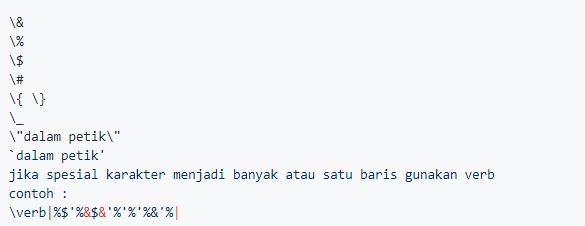
\includegraphics[width=0.70\textwidth]{figures/1.JPG}}
	\caption{Contoh Penggunaan Karakter Khusus}
	\label{KarakterKhusus}
\end{figure}


\section{Kode Program}
Agar kita dapat memasukan kode program, kita dapat menggunakan perintah \textit{lstlisting}. Perintah ini  berfungsi untuk memasukkan atau menambahkan kode program apapun ke dalam file yang terpisah. Untuk memasukan perintah \textit{lstlisting} kita perlu menulis parameter \textit{caption} dan \textit{label} untuk memberikan penjelasan keterangan kode program dan sebagai sumber referensi dari label kode program.

\lstinputlisting[caption=Menambahkan kode program,label={lst:kodeprogram}]{src/1/lstlisting.tex}

\section{Menambahkan Gambar}
Cara menambahkan gambar seperti pada listing \ref{lst:kodegambar}.
\lstinputlisting[caption=Contoh kode untuk menambahkan gambar,label={lst:kodegambar}]{src/1/figure.tex}


\section{Tabel}
Untuk dapat membuat tabel kita harus menggunakan perintah \textit{table}. Selain itu kita juga perlu menambahkan referensi pada tabel yang terdapat dalam kalimat berdasarkan labelnya. 

\section{Document class}

Pada dokumen Latex terdapat atau mempunyai beberapa struktur yang dicirikan dengan blok yang diberi apit oleh perintah begin dan end. Latex memberikan pilihan Class dokuman yang bisa di pakai, antara lain aadlah Book, Report, Article dan lain sebagainya. Class document book merupakan Class Document yang paling tepat untuk menulis, karena dapat mendukung table of contents yang dapat berfungsi langsung untuk generate daftar isi secara langsung.

Dalam memberikan penulisan judul pada format latex biasanya di letakkan pada awal document, untuk cara penulisan nya dapat dilakukan sebagai berikut:
\begin{enumerate}
  \item \textit{backslash} document class kurung kurawal a4papper, ukuran yang di inginkan tutup kurawal lalu report
  \item \textit{backslash} begin buka kurawal document tutup kurawal
  \item \textit{backslash} begin buka kurawal judul document tutup kurawal
  \item \textit{backslash} autor buka kurawal nama penulis tutup kurawal
  \item \textit{backslash} date buka kurawal tanggal pembuatan tutup kurawal
  \item \textit{backslash} maketitle
  \item \textit{backslash} and buka kurawal document tutup kurawal
\end{enumerate}

\section{Costum Command}
Sesuai  dengan  namanya Costum Command, dimana ke unggulan latex ada fitur yang satu ini, Pembuat dokumen ini dapat  membuat macro untuk kebutuhan yang sifatnya spesifik dan berulang-ulang, dimana costum cummad dapat melakukan tanda bintang berjejer sebagai penanda garis.





\section{Membuat Penomoran Referensi}
Disaat mengutip maupun menggunakan sanitasi diperkenankan untuk memberi keterangan referensi/sumber asal suatu kutipan/gagasan seperti pada gambar \ref{fig:contohpenomoranref}.
\begin{figure}[!htbp]
  \centering
  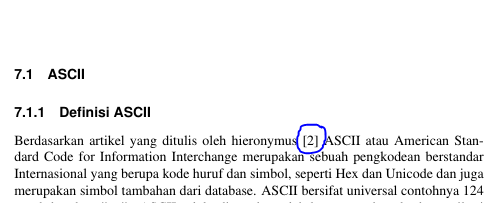
\includegraphics[width=.75\textwidth]{figures/contohpenomoranref.png}
  \caption{Ini adalah Contoh Penomoran Referensi}\label{fig:contohpenomoranref}
\end{figure}
\par Bagaimana cara membuatnya di Latex? berikut cara membuatnya:
\begin{enumerate}
  \item Cari materi yang akan dikutip melalui Google Scholar seperti pada gambar \ref{fig:scholar} ,
  \begin{figure}[!htbp]
  \centering
  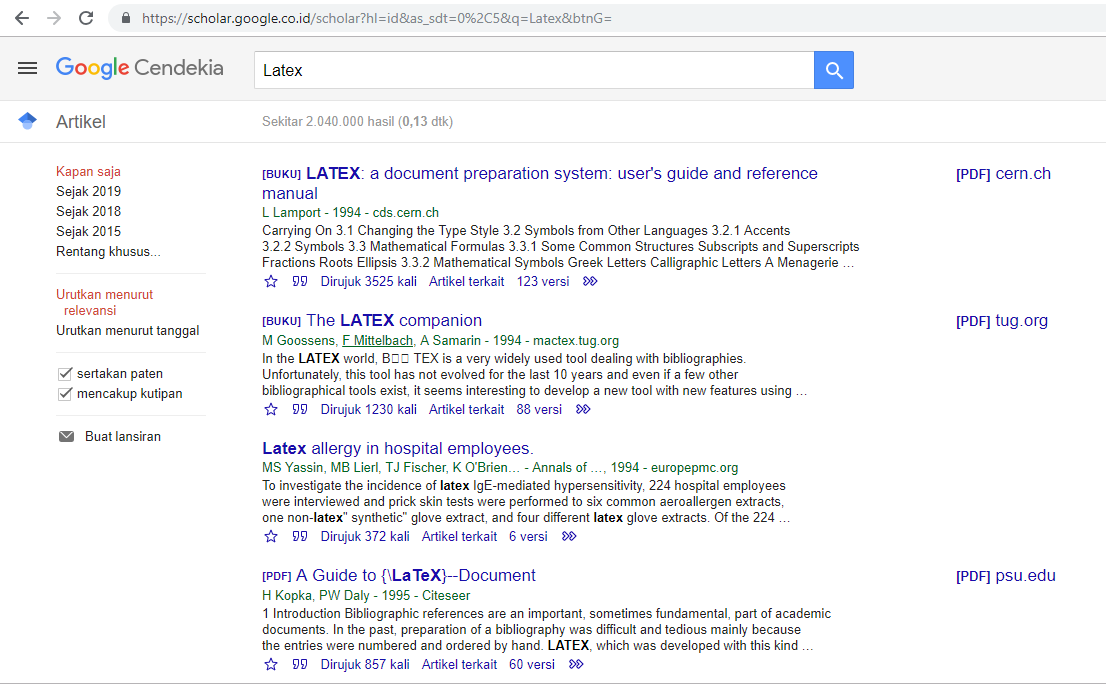
\includegraphics[width=.75\textwidth]{figures/scholar.png}
  \caption{Ini adalah Halaman Google Scholar}\label{fig:scholar}
\end{figure}
  \item Setelah selesai mengutip jangan lupa untuk mengambil script bibtexnya dengan cara klik pada tanda '' seperti pada gambar \ref{fig:awalbibtex},
  \begin{figure}[!htbp]
  \centering
  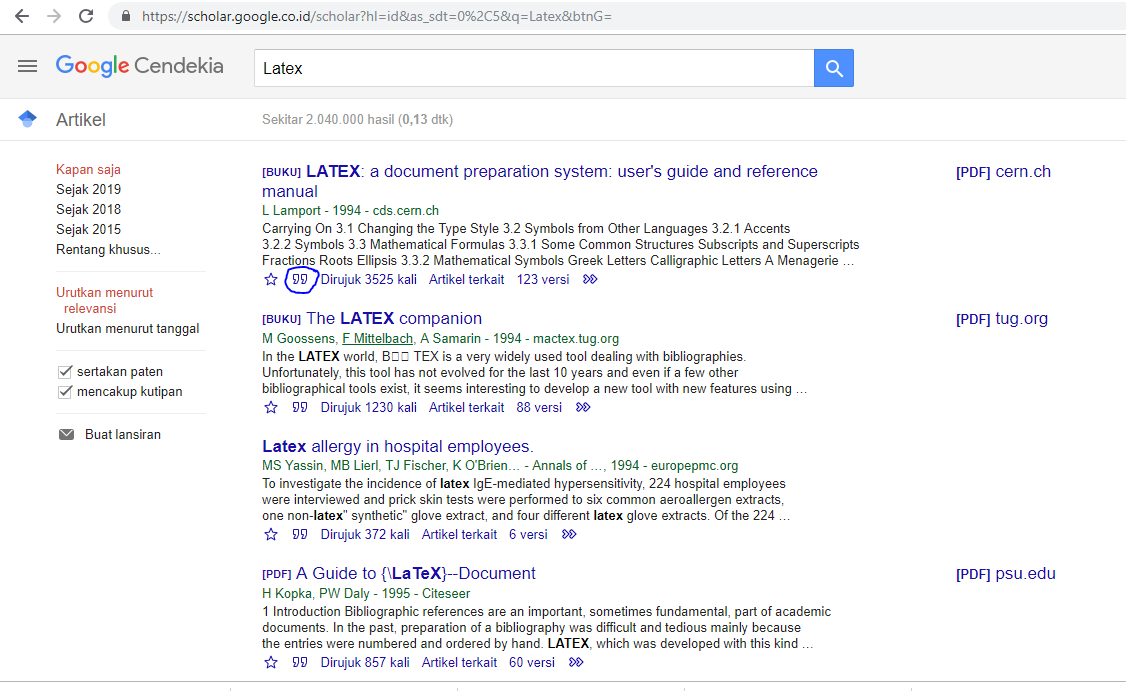
\includegraphics[width=.75\textwidth]{figures/awalbibtex.png}
  \caption{Ini adalah Tanda proses awal mengambil reference}\label{fig:awalbibtex}
\end{figure}
  \item Maka akan muncul seperti gambar \ref{fig:kutip}, lalu pilih Bibtex.
  \begin{figure}[!htbp]
  \centering
  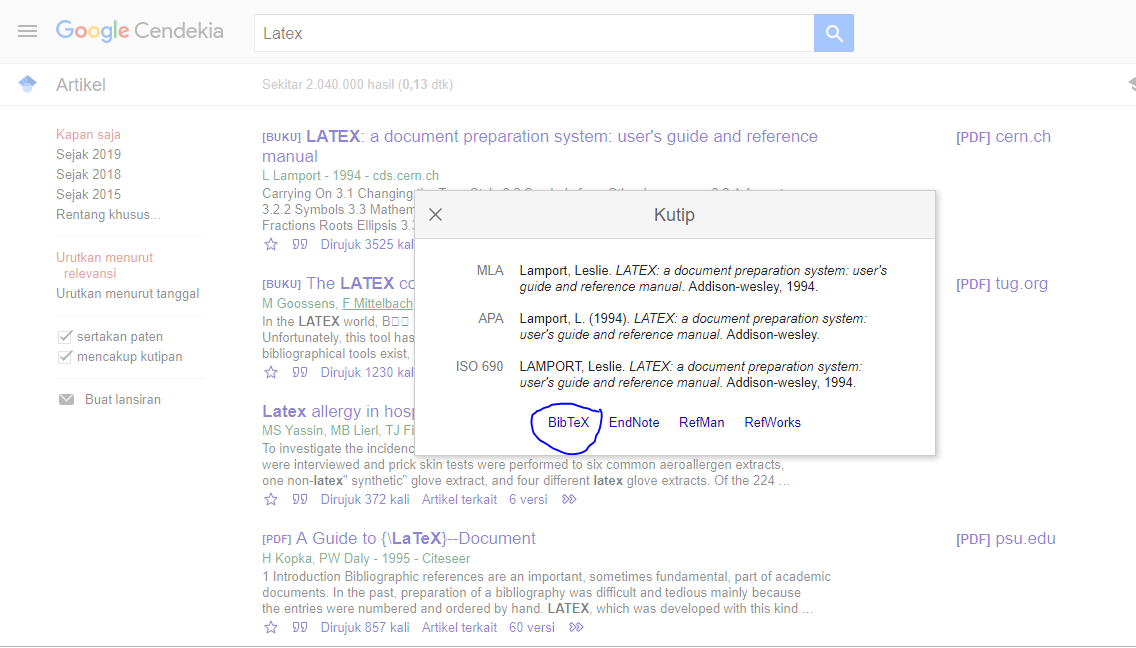
\includegraphics[width=.75\textwidth]{figures/kutip.png}
  \caption{Ini adalah Pilihan mengutip}\label{fig:kutip}
\end{figure}
  \item Setelah memilih Bibtex maka akan muncul script seperti pada gambar \ref{fig:scriptbibtex},
  \begin{figure}[!htbp]
  \centering
  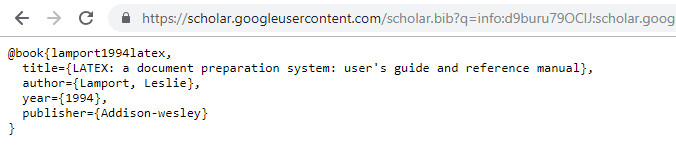
\includegraphics[width=.75\textwidth]{figures/scriptbibtex.png}
  \caption{Ini adalah Script BibTex}\label{fig:scriptbibtex}
\end{figure}
  \item Script tersebut dicopy pada direktori yang dikerjakan, khususnya pada bagian reference.bib seperti pada gambar \ref{fig:direktori} dan \ref{fig:reference} pada editor,
  \begin{figure}[!htbp]
  \centering
  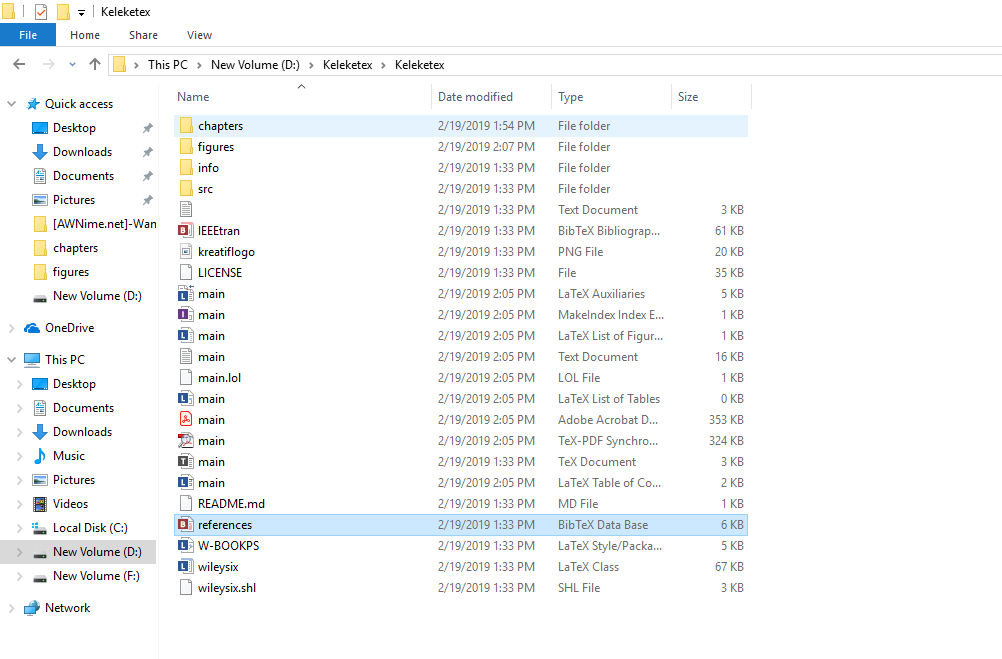
\includegraphics[width=.75\textwidth]{figures/direktori.png}
  \caption{Ini adalah Direktori pekerjaan}\label{fig:direktori}
\end{figure}
\begin{figure}[!htbp]
  \centering
  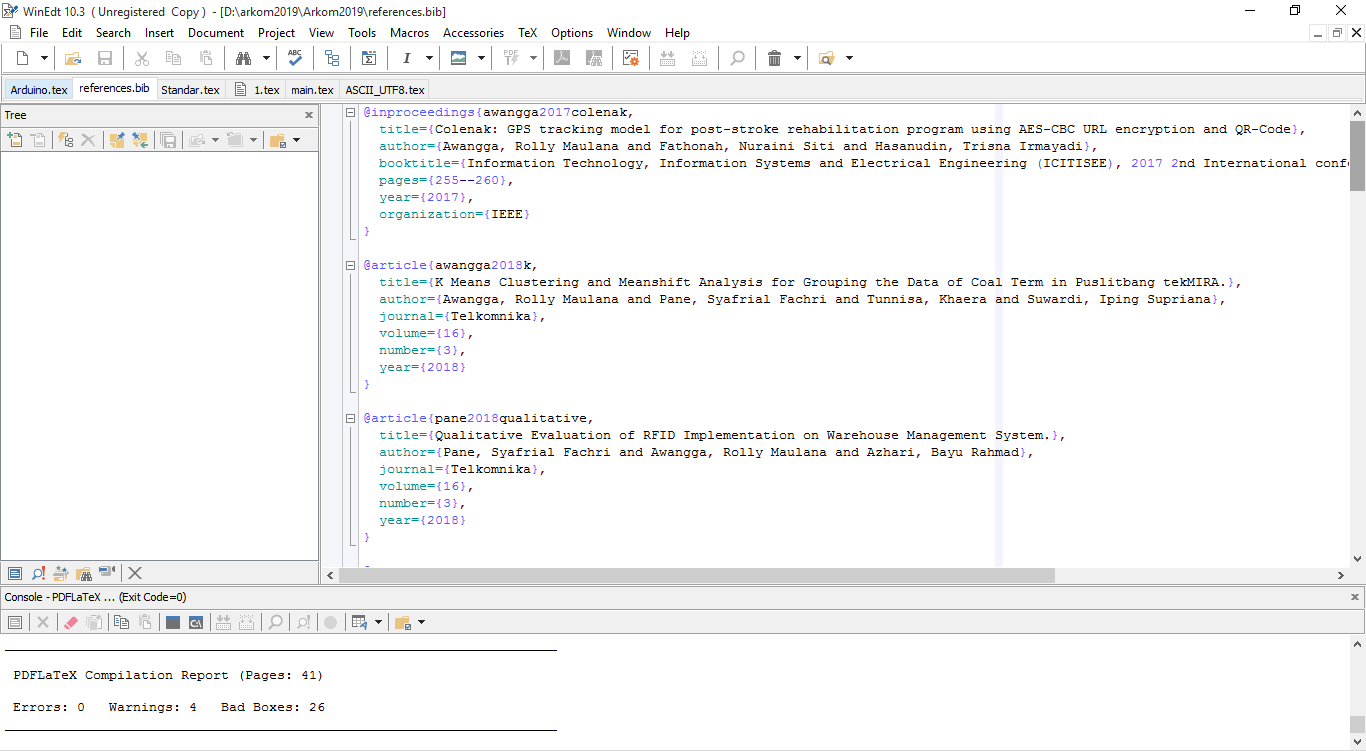
\includegraphics[width=.75\textwidth]{figures/reference.png}
  \caption{Ini adalah Reference.bib}\label{fig:reference}
\end{figure}
  \item Setelah dicopy, jangan lupa disave.
  \item Buka kembali pada lembar kerja yang sudah diberi kutipan/gagasan. Lalu tambahkan script setelah kutipan maka akan muncul seperti pada gambar \ref{fig:memilihsumber},
\lstinputlisting[caption=Penggunaan perintah cite untuk reference, label={Cite}]{src/1/reference.tex}
  \begin{figure}[!htbp]
  \centering
  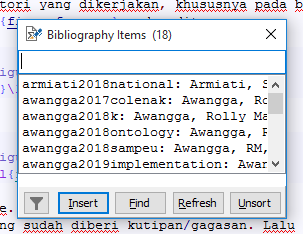
\includegraphics[width=.75\textwidth]{figures/memilihsumber.png}
  \caption{Ini adalah Proses pemilihan sumber}\label{fig:memilihsumber}
\end{figure}
  \item Pilih insert dan save.
  \item Untuk proses compilenya dilakukan 2 kali yaitu pada main.tex pilih Tex lalu pilih pdflatex dan Bibtex, dilakukan berulang minimal 3 kali compile. Seperti pada gambar \ref{fig:pdflatex} untuk pdflatex dan \ref{fig:bibtexx} untuk BibTex.
   \begin{figure}[!htbp]
  \centering
  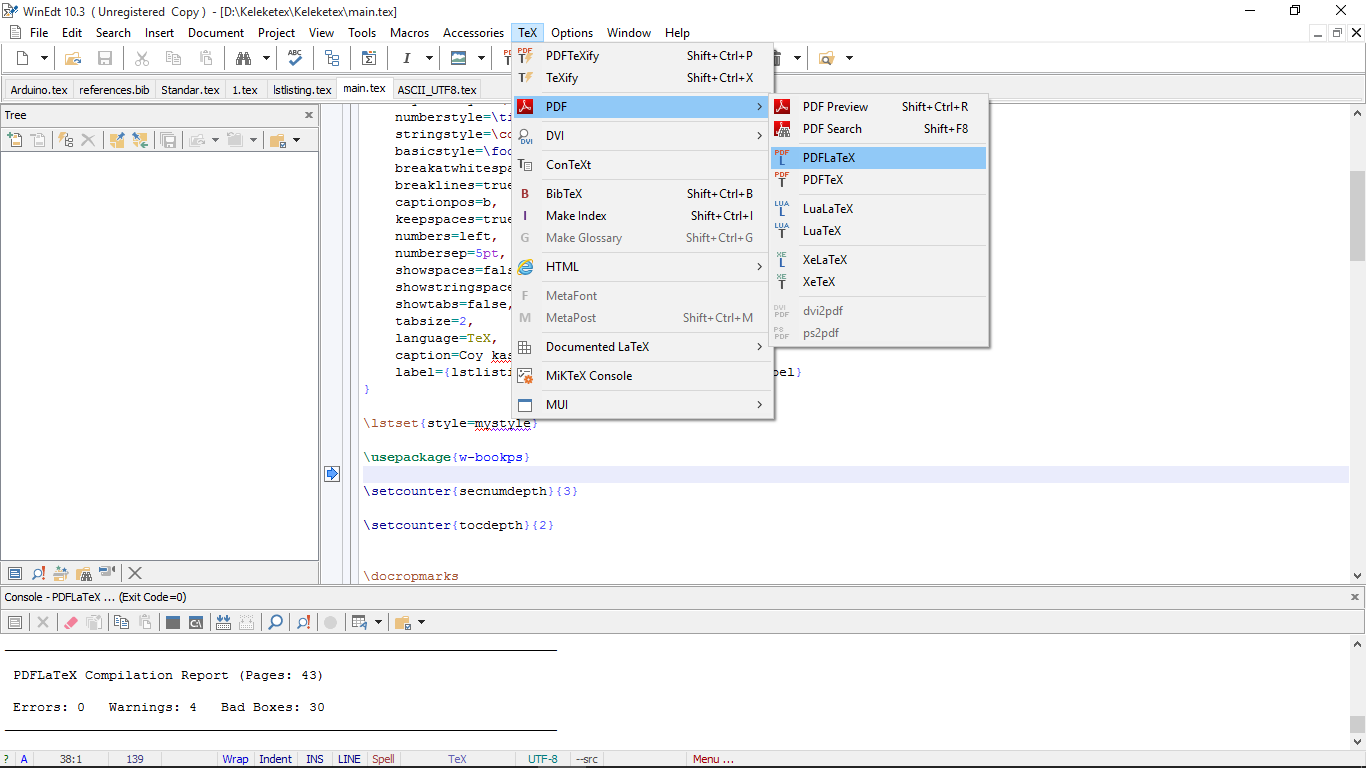
\includegraphics[width=.75\textwidth]{figures/pdflatex.png}
  \caption{Ini adalah Compile pdflatex}\label{fig:pdflatex}
\end{figure}
   \begin{figure}[!htbp]
  \centering
  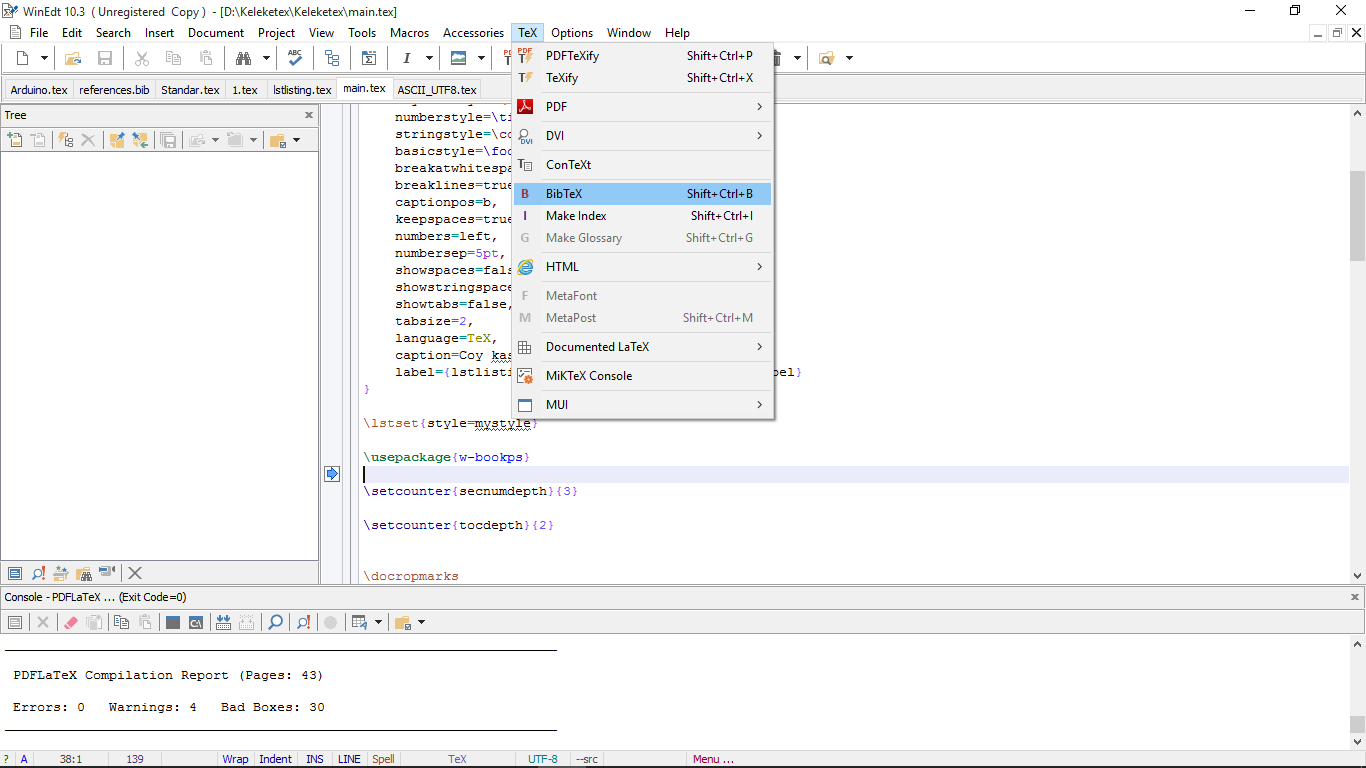
\includegraphics[width=.75\textwidth]{figures/bibtexx.png}
  \caption{Ini adalah Compile BibTex}\label{fig:bibtexx}
\end{figure}
\end{enumerate}

\section{Menambahkan Spesial Karakter}
cara memasukkan karakter spesial menggunakan listing \ref{lst:kodespesial}.
\lstinputlisting[caption=Contoh kode untuk menambahkan karakter spesial,label={lst:kodespesial}]{src/1/spesial.tex}




\chapter{Menambahkan Gambar}
\section{Perintah Navigasi}
Pastikan package ini sudah ada diawal code main.tex, jika belum, maka tambahkanlah:
\begin{lstlisting}
\usepackage{graphicx}
\end{lstlisting}

Lalu tambahkanlah code ini untuk memasukkan gambar
\begin{lstlisting}
\includegraphics[scale=0.8]{namafile}
\end{lstlisting}

Scaling berfungsi untuk mengatur size gambar sesuai dengan keinginan anda, 1.0 artinya original size, diatas itu untuk memperbesar, dibawah itu untuk memperkecil. Nama file nya tidak memerlukan ekstensi, tetapi nama file nya jangan memakai spasi, karena tidak sesuai dengan standar pengkodean. 

\chapter{Menambahkan Chapter}
\section{Membuat Rumus dengan LaTex}
Sebagai aplikasi editor pengolah dokumen, LATEX memiliki kemampuan yang mampu menghasilkan dokumen berisi notasi-notasi matematis. Agar dapat menghasilkan dokumen yang berisikan notasi-notasi matematis maka kita harus berada dalam \textit{Mathematics Environtment}. Terdapat beberapa perintah yang bisa digunakan dalam membuat rumus pada latex. Kita dapat menggunakan perintah \textit{equation}, \textit{displaymath} ataupun menggunakan \$. Kita juga dapat menyelipkan rumus didalam suatu kalimat di sebuah paragraf dengan menggunakan perintah \$\$.

\section{Penulisan Notasi Matematika}
Pada latex kita dapat menuliskan suatu notasi matematika yang cukup panjang dalam suatu paragraf baru. Penulisan Notasi Matematika dalam suatu paragraf dapat dilihat pada listing \ref{lst:notasi_paragraf}.
\lstinputlisting[caption=Notasi Matematika Dalam Paragraf,label={lst:notasi_paragraf}]{src/3/notasi1.tex}

\section{Font Dalam Notasi Matematika}
Ada beberapa perintah pada yang dapat digunakan untuk mengubah jenis font notasi matematis dalam latex. Beberapa perintah tersebut dapat kita lihat pada listing \ref{lst:fontmath}.
\lstinputlisting[caption=Jenis Font Matematis,label={lst:fontmath}]{src/3/font.tex}

Hasil output : 

$\mathrm{x y z}$

$\mathsf{x y z}$

$\mathtt{x y z}$

$\mathit{x y z}$

$\mathbf{x y z}$

\section{Rumus Dasar}
Rumus dasar ini terdiri dari 3 notasi yaitu penjumlahan, pengurangan, dan perkalian. Contoh kode untuk rumus dasar bisa dilihat pada listing \ref{lst:rumus_dasar}.
\lstinputlisting[caption=Penggunaan Rumus Dasar,label={lst:rumus_dasar}]{src/1/rumus_dasar.tex}
Hasil output:

$$ a+b$$

$$ a-b$$

$$ a \times b$$

\subsection{Rumus Pecahan}
Rumus pecahan yang dimaksud adalah notasi per pada pembagian. Contoh kode untuk rumus pecahan bisa dilihat pada listing \ref{lst:rumus_pecahan}.
\lstinputlisting[caption=Penggunaan Rumus Pecahan,label={lst:rumus_pecahan}]{src/1/rumus_pecahan.tex}
Hasil output:

$$ a/b$$

$$ \frac {a}{b}$$

\subsection{Rumus Akar}
Rumus akar dapat dilihat pada listing \ref{lst:rumus_akar}.
\ref{lst:rumus_akar}.
\lstinputlisting[caption=Penggunaan Rumus Akar,label={lst:rumus_akar}]{src/1/rumus_akar.tex}
Hasil output:

$$ \sqrt[a]{b}$$

$$ \sqrt{\sqrt{a}}$$

\section{Perumusan Menggunakan Superscripts dan Subscripts}
Penulisan \textit{Supserscripts} dan \textit{Subscripts} biasanya digunakan untuk membuat sebuah rumus dengan menghasilkan pangkat diatas dan pangkat dibawah pada suatu rumus. Cara penulisan penggunaan ini adalah dengan menggunakan perintah \textbf{sp} dan perintah \textbf{sb}. Untuk contoh penerapan perintah \textit{Supserscripts} dan \textit{Subscripts} dapat kita lihat pada listing \ref{lst:sp1}.

\lstinputlisting[caption=Penggunaan Supersripts dan Subscripts,label={lst:sp1}]{src/3/sp1.tex}

Hasil output :

\begin{displaymath}
y = x\sb{1}\sp{2} + x\sb{2}\sp{2}
\end{displaymath}

Atau kita juga dapat menggunakan perintah lain seperti pada listing \ref{lst:sp2}.

\lstinputlisting[caption=Perintah Pada Superscripts dan Subscripts,label={lst:sp2}]{src/3/sp2.tex}

Hasil output :

\begin{displaymath}
f(x) = e^{x_1}
\end{displaymath}

\section {Perumusan Array dan Matriks}
Dalam LaTex, kita dapat menuliskan rumus sebuah array pada environment \textbf{tabular}. Perintah untuk membuat array dan matriks dapat kita lihat pada listing \ref{lst:array}.
\lstinputlisting[caption=Penulisan Array atau Matriks,label={lst:array}]{src/3/array.tex}

Hasil output :

\begin{displaymath}
\left (
\begin{array}{rrr}
0 & 55 & 23 \\
34 & -83 & 68 \end{array}
\right )
\end{displaymath}

Ada beberapa hal yang perlu kita ketahui dalam penulisan rumus array atau matriks ini :
\begin{itemize}
\item Penulisan array memiliki kesamaan seperti saat membuat format tabel
\item Perintah \textbf{"rrr"} berfungsi untuk menentukan posisi dari masing-masing komponen matriks tersebut
\item Tanda kurung kurawal "( )" berfungsi untuk mendefinisikan bagian kurung buka dan kurung tutup pada sebuah matriks  
\end{itemize}

\section{Perumusan Vektor}
Dalam LaTex, perumusan dengan format \textit{vektor} kita dapat menuliskannya dengan perintah seperti pada listing \ref{lst:vektor}.
\lstinputlisting[caption=Penulisan Vektor,label={lst:vektor}]{src/3/vektor.tex} 

Contoh kita akan mengubah variabel \textit{x} kedalam satuan vektor. Maka hasil outputnya adalah :
\begin{displaymath}
\vec{x} = a + b
\end{displaymath} 

\section{Kombinasi Penggunaan Rumus}
Pada section ini kita akan mempelajari bagaimana mengkombinasikan sebuah rumus dari penulisan dasar rumus Subscript, Superscript, Akar Pangkat, Pecahan dan sejenisnya. Contoh pertama dapat kita lihat pada listing \ref{lst:sigma}.
\lstinputlisting[caption=Contoh Kombinasi Rumus Sigma,label={lst:sigma}]{src/3/sigma.tex}

Hasil output :

$$\sum^{\infty}_{n=1} \frac{1}{n}$$

Setelah melihat salah satu penggunaan kombinasi rumus diatas kita bisa melakukan kombinasi rumus lainnya. Seperti yang akan diperlihatkan pada listing \ref{lst:kombinasi}

\lstinputlisting[caption=Contoh Kombinasi Rumus,label={lst:kombinasi}]{src/3/kombinasi.tex}

Hasil output :
\begin{enumerate}
\item $\sqrt{ \frac{a^2}{3b^3+1}}$
\item $\lim_{n \to \infty} \frac{1}{n}=0$
\item $\int^b_a x^2 \, dx$
\item $\lim \limits_{n \to \infty} \frac{1}{n}=0$
\item $\int \limits^b_a x^2 \, dx$
\item $\sum \limits^{\infty}_{n=1} \frac{1}{n}$
\end{enumerate}









\bibliographystyle{IEEEtran} 
\bibliography{references}


\printindex
\end{document}

